\documentclass[twoside]{book}

% Packages required by doxygen
\usepackage{fixltx2e}
\usepackage{calc}
\usepackage{doxygen}
\usepackage[export]{adjustbox} % also loads graphicx
\usepackage{graphicx}
\usepackage[utf8]{inputenc}
\usepackage{makeidx}
\usepackage{multicol}
\usepackage{multirow}
\PassOptionsToPackage{warn}{textcomp}
\usepackage{textcomp}
\usepackage[nointegrals]{wasysym}
\usepackage[table]{xcolor}

% Font selection
\usepackage[T1]{fontenc}
\usepackage[scaled=.90]{helvet}
\usepackage{courier}
\usepackage{amssymb}
\usepackage{sectsty}
\renewcommand{\familydefault}{\sfdefault}
\allsectionsfont{%
  \fontseries{bc}\selectfont%
  \color{darkgray}%
}
\renewcommand{\DoxyLabelFont}{%
  \fontseries{bc}\selectfont%
  \color{darkgray}%
}
\newcommand{\+}{\discretionary{\mbox{\scriptsize$\hookleftarrow$}}{}{}}

% Page & text layout
\usepackage{geometry}
\geometry{%
  a4paper,%
  top=2.5cm,%
  bottom=2.5cm,%
  left=2.5cm,%
  right=2.5cm%
}
\tolerance=750
\hfuzz=15pt
\hbadness=750
\setlength{\emergencystretch}{15pt}
\setlength{\parindent}{0cm}
\setlength{\parskip}{0.2cm}
\makeatletter
\renewcommand{\paragraph}{%
  \@startsection{paragraph}{4}{0ex}{-1.0ex}{1.0ex}{%
    \normalfont\normalsize\bfseries\SS@parafont%
  }%
}
\renewcommand{\subparagraph}{%
  \@startsection{subparagraph}{5}{0ex}{-1.0ex}{1.0ex}{%
    \normalfont\normalsize\bfseries\SS@subparafont%
  }%
}
\makeatother

% Headers & footers
\usepackage{fancyhdr}
\pagestyle{fancyplain}
\fancyhead[LE]{\fancyplain{}{\bfseries\thepage}}
\fancyhead[CE]{\fancyplain{}{}}
\fancyhead[RE]{\fancyplain{}{\bfseries\leftmark}}
\fancyhead[LO]{\fancyplain{}{\bfseries\rightmark}}
\fancyhead[CO]{\fancyplain{}{}}
\fancyhead[RO]{\fancyplain{}{\bfseries\thepage}}
\fancyfoot[LE]{\fancyplain{}{}}
\fancyfoot[CE]{\fancyplain{}{}}
\fancyfoot[RE]{\fancyplain{}{\bfseries\scriptsize Generated by Doxygen }}
\fancyfoot[LO]{\fancyplain{}{\bfseries\scriptsize Generated by Doxygen }}
\fancyfoot[CO]{\fancyplain{}{}}
\fancyfoot[RO]{\fancyplain{}{}}
\renewcommand{\footrulewidth}{0.4pt}
\renewcommand{\chaptermark}[1]{%
  \markboth{#1}{}%
}
\renewcommand{\sectionmark}[1]{%
  \markright{\thesection\ #1}%
}

% Indices & bibliography
\usepackage{natbib}
\usepackage[titles]{tocloft}
\setcounter{tocdepth}{3}
\setcounter{secnumdepth}{5}
\makeindex

% Hyperlinks (required, but should be loaded last)
\usepackage{ifpdf}
\ifpdf
  \usepackage[pdftex,pagebackref=true]{hyperref}
\else
  \usepackage[ps2pdf,pagebackref=true]{hyperref}
\fi
\hypersetup{%
  colorlinks=true,%
  linkcolor=blue,%
  citecolor=blue,%
  unicode%
}

% Custom commands
\newcommand{\clearemptydoublepage}{%
  \newpage{\pagestyle{empty}\cleardoublepage}%
}

\usepackage{caption}
\captionsetup{labelsep=space,justification=centering,font={bf},singlelinecheck=off,skip=4pt,position=top}

%===== C O N T E N T S =====

\begin{document}

% Titlepage & ToC
\hypersetup{pageanchor=false,
             bookmarks=true,
             bookmarksnumbered=true,
             pdfencoding=unicode
            }
\pagenumbering{roman}
\begin{titlepage}
\vspace*{7cm}
\begin{center}%
{\Large My Project }\\
\vspace*{1cm}
{\large Generated by Doxygen 1.8.11}\\
\end{center}
\end{titlepage}
\clearemptydoublepage
\tableofcontents
\clearemptydoublepage
\pagenumbering{arabic}
\hypersetup{pageanchor=true}

%--- Begin generated contents ---
\chapter{Hierarchical Index}
\section{Class Hierarchy}
This inheritance list is sorted roughly, but not completely, alphabetically\+:\begin{DoxyCompactList}
\item Message\begin{DoxyCompactList}
\item \contentsline{section}{machines\+:\+:Machine}{\pageref{classmachines_1_1Machine}}{}
\item \contentsline{section}{machines\+:\+:machinelist}{\pageref{classmachines_1_1machinelist}}{}
\end{DoxyCompactList}
\item \contentsline{section}{Prototype}{\pageref{classPrototype}}{}
\begin{DoxyCompactList}
\item \contentsline{section}{Machinetype1}{\pageref{classMachinetype1}}{}
\item \contentsline{section}{Machinetype2}{\pageref{classMachinetype2}}{}
\end{DoxyCompactList}
\item \contentsline{section}{machines\+:\+:Static\+Descriptor\+Initializer\+\_\+\+Machine\+\_\+2eproto}{\pageref{structmachines_1_1StaticDescriptorInitializer__Machine__2eproto}}{}
\end{DoxyCompactList}

\chapter{Class Index}
\section{Class List}
Here are the classes, structs, unions and interfaces with brief descriptions\+:\begin{DoxyCompactList}
\item\contentsline{section}{\hyperlink{classmachines_1_1Machine}{machines\+::\+Machine} }{\pageref{classmachines_1_1Machine}}{}
\item\contentsline{section}{\hyperlink{classmachines_1_1machinelist}{machines\+::machinelist} }{\pageref{classmachines_1_1machinelist}}{}
\item\contentsline{section}{\hyperlink{classMachinetype1}{Machinetype1} }{\pageref{classMachinetype1}}{}
\item\contentsline{section}{\hyperlink{classMachinetype2}{Machinetype2} }{\pageref{classMachinetype2}}{}
\item\contentsline{section}{\hyperlink{classPrototype}{Prototype} \\*\hyperlink{classPrototype}{Prototype} class }{\pageref{classPrototype}}{}
\item\contentsline{section}{\hyperlink{structmachines_1_1StaticDescriptorInitializer__Machine__2eproto}{machines\+::\+Static\+Descriptor\+Initializer\+\_\+\+Machine\+\_\+2eproto} }{\pageref{structmachines_1_1StaticDescriptorInitializer__Machine__2eproto}}{}
\end{DoxyCompactList}

\chapter{Class Documentation}
\hypertarget{classmachines_1_1Machine}{}\section{machines\+:\+:Machine Class Reference}
\label{classmachines_1_1Machine}\index{machines\+::\+Machine@{machines\+::\+Machine}}
Inheritance diagram for machines\+:\+:Machine\+:\begin{figure}[H]
\begin{center}
\leavevmode
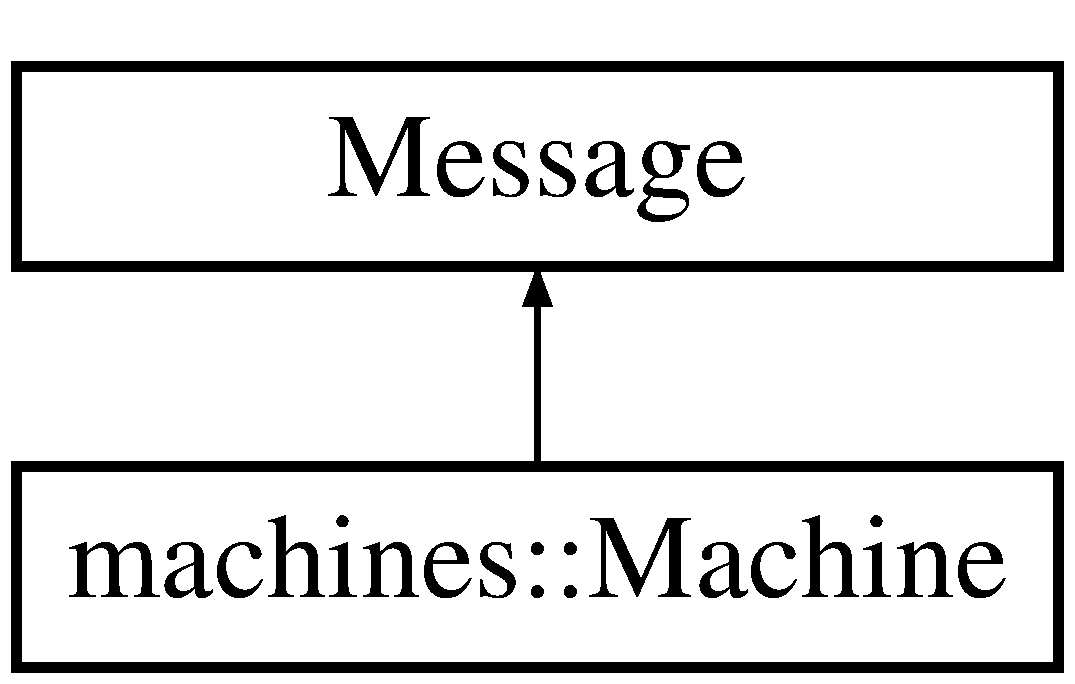
\includegraphics[height=2.000000cm]{classmachines_1_1Machine}
\end{center}
\end{figure}
\subsection*{Public Member Functions}
\begin{DoxyCompactItemize}
\item 
{\bfseries Machine} (const \hyperlink{classmachines_1_1Machine}{Machine} \&from)\hypertarget{classmachines_1_1Machine_a4bc25165182e6a979ef514463749076e}{}\label{classmachines_1_1Machine_a4bc25165182e6a979ef514463749076e}

\item 
\hyperlink{classmachines_1_1Machine}{Machine} \& {\bfseries operator=} (const \hyperlink{classmachines_1_1Machine}{Machine} \&from)\hypertarget{classmachines_1_1Machine_a446fbdac340914a6706dfe3251d7e9f7}{}\label{classmachines_1_1Machine_a446fbdac340914a6706dfe3251d7e9f7}

\item 
const \+::google\+::protobuf\+::\+Unknown\+Field\+Set \& {\bfseries unknown\+\_\+fields} () const \hypertarget{classmachines_1_1Machine_a253de277819734acf7ddc3669626fe0c}{}\label{classmachines_1_1Machine_a253de277819734acf7ddc3669626fe0c}

\item 
inline\+::google\+::protobuf\+::\+Unknown\+Field\+Set $\ast$ {\bfseries mutable\+\_\+unknown\+\_\+fields} ()\hypertarget{classmachines_1_1Machine_aa44fa140cc57ec8ce33d85d77444570a}{}\label{classmachines_1_1Machine_aa44fa140cc57ec8ce33d85d77444570a}

\item 
void {\bfseries Swap} (\hyperlink{classmachines_1_1Machine}{Machine} $\ast$other)\hypertarget{classmachines_1_1Machine_aa4faae554cfeeb3c4e247822e203186d}{}\label{classmachines_1_1Machine_aa4faae554cfeeb3c4e247822e203186d}

\item 
\hyperlink{classmachines_1_1Machine}{Machine} $\ast$ {\bfseries New} () const \hypertarget{classmachines_1_1Machine_ae21b376d3ca27fb1998a640cf3c5b466}{}\label{classmachines_1_1Machine_ae21b376d3ca27fb1998a640cf3c5b466}

\item 
\hyperlink{classmachines_1_1Machine}{Machine} $\ast$ {\bfseries New} (\+::google\+::protobuf\+::\+Arena $\ast$arena) const \hypertarget{classmachines_1_1Machine_ac68514d217a1622798bb41a662b9cf41}{}\label{classmachines_1_1Machine_ac68514d217a1622798bb41a662b9cf41}

\item 
void {\bfseries Copy\+From} (const \+::google\+::protobuf\+::\+Message \&from)\hypertarget{classmachines_1_1Machine_acea5a9547edd90825e68d4d80e9cb4ed}{}\label{classmachines_1_1Machine_acea5a9547edd90825e68d4d80e9cb4ed}

\item 
void {\bfseries Merge\+From} (const \+::google\+::protobuf\+::\+Message \&from)\hypertarget{classmachines_1_1Machine_aab1a9f0422cb52ca5781abfe38dc6aa8}{}\label{classmachines_1_1Machine_aab1a9f0422cb52ca5781abfe38dc6aa8}

\item 
void {\bfseries Copy\+From} (const \hyperlink{classmachines_1_1Machine}{Machine} \&from)\hypertarget{classmachines_1_1Machine_a1ef5ec4d9c03347fafcbe852c8713810}{}\label{classmachines_1_1Machine_a1ef5ec4d9c03347fafcbe852c8713810}

\item 
void {\bfseries Merge\+From} (const \hyperlink{classmachines_1_1Machine}{Machine} \&from)\hypertarget{classmachines_1_1Machine_a110d8b5bd9c882d5ce284408ce2360fc}{}\label{classmachines_1_1Machine_a110d8b5bd9c882d5ce284408ce2360fc}

\item 
void {\bfseries Clear} ()\hypertarget{classmachines_1_1Machine_a83f013a6037eb1a0f4bb8f6480fcf203}{}\label{classmachines_1_1Machine_a83f013a6037eb1a0f4bb8f6480fcf203}

\item 
bool {\bfseries Is\+Initialized} () const \hypertarget{classmachines_1_1Machine_ac58156f3089f29f3db2652fd9e0bb5a9}{}\label{classmachines_1_1Machine_ac58156f3089f29f3db2652fd9e0bb5a9}

\item 
int {\bfseries Byte\+Size} () const \hypertarget{classmachines_1_1Machine_afadfed0c3b2e6bf73fd6b67e563cf12b}{}\label{classmachines_1_1Machine_afadfed0c3b2e6bf73fd6b67e563cf12b}

\item 
bool {\bfseries Merge\+Partial\+From\+Coded\+Stream} (\+::google\+::protobuf\+::io\+::\+Coded\+Input\+Stream $\ast$input)\hypertarget{classmachines_1_1Machine_a905f5a8e9551450e7ed999709c0822ad}{}\label{classmachines_1_1Machine_a905f5a8e9551450e7ed999709c0822ad}

\item 
void {\bfseries Serialize\+With\+Cached\+Sizes} (\+::google\+::protobuf\+::io\+::\+Coded\+Output\+Stream $\ast$output) const \hypertarget{classmachines_1_1Machine_a184c7d162b62e3a1c786a85e120447a7}{}\label{classmachines_1_1Machine_a184c7d162b62e3a1c786a85e120447a7}

\item 
\+::google\+::protobuf\+::uint8 $\ast$ {\bfseries Serialize\+With\+Cached\+Sizes\+To\+Array} (\+::google\+::protobuf\+::uint8 $\ast$output) const \hypertarget{classmachines_1_1Machine_a34a75799ebb229a2d1661e2607cd1b3f}{}\label{classmachines_1_1Machine_a34a75799ebb229a2d1661e2607cd1b3f}

\item 
int {\bfseries Get\+Cached\+Size} () const \hypertarget{classmachines_1_1Machine_a648152e9c2f16354f92ca10795e60597}{}\label{classmachines_1_1Machine_a648152e9c2f16354f92ca10795e60597}

\item 
\+::google\+::protobuf\+::\+Metadata {\bfseries Get\+Metadata} () const \hypertarget{classmachines_1_1Machine_a3421c3b065c0c0ca06f9b409511770fb}{}\label{classmachines_1_1Machine_a3421c3b065c0c0ca06f9b409511770fb}

\item 
bool {\bfseries has\+\_\+type} () const \hypertarget{classmachines_1_1Machine_a42b635e2648adf6cd3345b64cf91e822}{}\label{classmachines_1_1Machine_a42b635e2648adf6cd3345b64cf91e822}

\item 
void {\bfseries clear\+\_\+type} ()\hypertarget{classmachines_1_1Machine_ae9a2cbfcf6fc27cc8932715150bc08de}{}\label{classmachines_1_1Machine_ae9a2cbfcf6fc27cc8932715150bc08de}

\item 
const \+::std\+::string \& {\bfseries type} () const \hypertarget{classmachines_1_1Machine_ad12df0c21c6d063e3f0789840f7d1a7b}{}\label{classmachines_1_1Machine_ad12df0c21c6d063e3f0789840f7d1a7b}

\item 
void {\bfseries set\+\_\+type} (const \+::std\+::string \&value)\hypertarget{classmachines_1_1Machine_a1afeaa8b127c45f9cd438ae28391c5b3}{}\label{classmachines_1_1Machine_a1afeaa8b127c45f9cd438ae28391c5b3}

\item 
void {\bfseries set\+\_\+type} (const char $\ast$value)\hypertarget{classmachines_1_1Machine_aa03348ee860c5a2551c2ae286a1d63f1}{}\label{classmachines_1_1Machine_aa03348ee860c5a2551c2ae286a1d63f1}

\item 
void {\bfseries set\+\_\+type} (const char $\ast$value, size\+\_\+t size)\hypertarget{classmachines_1_1Machine_a1a82c2df5be926042e58923a008d7871}{}\label{classmachines_1_1Machine_a1a82c2df5be926042e58923a008d7871}

\item 
\+::std\+::string $\ast$ {\bfseries mutable\+\_\+type} ()\hypertarget{classmachines_1_1Machine_ac246c53f1de5a23ca0cdce8c5846a0f9}{}\label{classmachines_1_1Machine_ac246c53f1de5a23ca0cdce8c5846a0f9}

\item 
\+::std\+::string $\ast$ {\bfseries release\+\_\+type} ()\hypertarget{classmachines_1_1Machine_adcd1d15e61c2583c8060ab510117bb27}{}\label{classmachines_1_1Machine_adcd1d15e61c2583c8060ab510117bb27}

\item 
void {\bfseries set\+\_\+allocated\+\_\+type} (\+::std\+::string $\ast$type)\hypertarget{classmachines_1_1Machine_a6a918dec3c402fc8046d1c7390106b0d}{}\label{classmachines_1_1Machine_a6a918dec3c402fc8046d1c7390106b0d}

\item 
bool {\bfseries has\+\_\+id} () const \hypertarget{classmachines_1_1Machine_af0d71aff9fdeaac6fc24a2de203c69a9}{}\label{classmachines_1_1Machine_af0d71aff9fdeaac6fc24a2de203c69a9}

\item 
void {\bfseries clear\+\_\+id} ()\hypertarget{classmachines_1_1Machine_a11ca5c940ac36652211bbd2e05ca845a}{}\label{classmachines_1_1Machine_a11ca5c940ac36652211bbd2e05ca845a}

\item 
const \+::std\+::string \& {\bfseries id} () const \hypertarget{classmachines_1_1Machine_ac8fec633a49ac84d9ab272d3b09a81a1}{}\label{classmachines_1_1Machine_ac8fec633a49ac84d9ab272d3b09a81a1}

\item 
void {\bfseries set\+\_\+id} (const \+::std\+::string \&value)\hypertarget{classmachines_1_1Machine_af6554eeb773c2b46d2db81ba718f9a67}{}\label{classmachines_1_1Machine_af6554eeb773c2b46d2db81ba718f9a67}

\item 
void {\bfseries set\+\_\+id} (const char $\ast$value)\hypertarget{classmachines_1_1Machine_a738eb71505d36730d0b4a1579d5a2d9e}{}\label{classmachines_1_1Machine_a738eb71505d36730d0b4a1579d5a2d9e}

\item 
void {\bfseries set\+\_\+id} (const char $\ast$value, size\+\_\+t size)\hypertarget{classmachines_1_1Machine_ac1ce9e88b4dac3c067816ccecd3b7ba4}{}\label{classmachines_1_1Machine_ac1ce9e88b4dac3c067816ccecd3b7ba4}

\item 
\+::std\+::string $\ast$ {\bfseries mutable\+\_\+id} ()\hypertarget{classmachines_1_1Machine_af6736b89d275d827f10e41a8e15c81dc}{}\label{classmachines_1_1Machine_af6736b89d275d827f10e41a8e15c81dc}

\item 
\+::std\+::string $\ast$ {\bfseries release\+\_\+id} ()\hypertarget{classmachines_1_1Machine_a73c06da38aad3f51f2affcf17a93ebae}{}\label{classmachines_1_1Machine_a73c06da38aad3f51f2affcf17a93ebae}

\item 
void {\bfseries set\+\_\+allocated\+\_\+id} (\+::std\+::string $\ast$id)\hypertarget{classmachines_1_1Machine_aa1fcfbf21ecf6aea87c258201475c43b}{}\label{classmachines_1_1Machine_aa1fcfbf21ecf6aea87c258201475c43b}

\end{DoxyCompactItemize}
\subsection*{Static Public Member Functions}
\begin{DoxyCompactItemize}
\item 
static const \+::google\+::protobuf\+::\+Descriptor $\ast$ {\bfseries descriptor} ()\hypertarget{classmachines_1_1Machine_afd031b5e971083f0e7c0aaaa3558d36f}{}\label{classmachines_1_1Machine_afd031b5e971083f0e7c0aaaa3558d36f}

\item 
static const \hyperlink{classmachines_1_1Machine}{Machine} \& {\bfseries default\+\_\+instance} ()\hypertarget{classmachines_1_1Machine_ac32386f09022b17269958601d93f58b5}{}\label{classmachines_1_1Machine_ac32386f09022b17269958601d93f58b5}

\end{DoxyCompactItemize}
\subsection*{Static Public Attributes}
\begin{DoxyCompactItemize}
\item 
static const int {\bfseries k\+T\+Y\+P\+E\+Field\+Number} = 1\hypertarget{classmachines_1_1Machine_a841bad16ef5c0d88e5c06545215db687}{}\label{classmachines_1_1Machine_a841bad16ef5c0d88e5c06545215db687}

\item 
static const int {\bfseries k\+I\+D\+Field\+Number} = 2\hypertarget{classmachines_1_1Machine_aed921813c3247bfc663af77808511137}{}\label{classmachines_1_1Machine_aed921813c3247bfc663af77808511137}

\end{DoxyCompactItemize}
\subsection*{Friends}
\begin{DoxyCompactItemize}
\item 
void {\bfseries protobuf\+\_\+\+Add\+Desc\+\_\+\+Machine\+\_\+2eproto} ()\hypertarget{classmachines_1_1Machine_ab588f006d8ec48121b79de6050e1f8a3}{}\label{classmachines_1_1Machine_ab588f006d8ec48121b79de6050e1f8a3}

\item 
void {\bfseries protobuf\+\_\+\+Assign\+Desc\+\_\+\+Machine\+\_\+2eproto} ()\hypertarget{classmachines_1_1Machine_a4615177ebb310c1aa54ad33e1bf40d43}{}\label{classmachines_1_1Machine_a4615177ebb310c1aa54ad33e1bf40d43}

\item 
void {\bfseries protobuf\+\_\+\+Shutdown\+File\+\_\+\+Machine\+\_\+2eproto} ()\hypertarget{classmachines_1_1Machine_abdd3c852817cdd7a28aeb79f6757bde2}{}\label{classmachines_1_1Machine_abdd3c852817cdd7a28aeb79f6757bde2}

\end{DoxyCompactItemize}


The documentation for this class was generated from the following files\+:\begin{DoxyCompactItemize}
\item 
Machine.\+pb.\+h\item 
Machine.\+pb.\+cc\end{DoxyCompactItemize}

\hypertarget{classmachines_1_1machinelist}{}\section{machines\+:\+:machinelist Class Reference}
\label{classmachines_1_1machinelist}\index{machines\+::machinelist@{machines\+::machinelist}}
Inheritance diagram for machines\+:\+:machinelist\+:\begin{figure}[H]
\begin{center}
\leavevmode
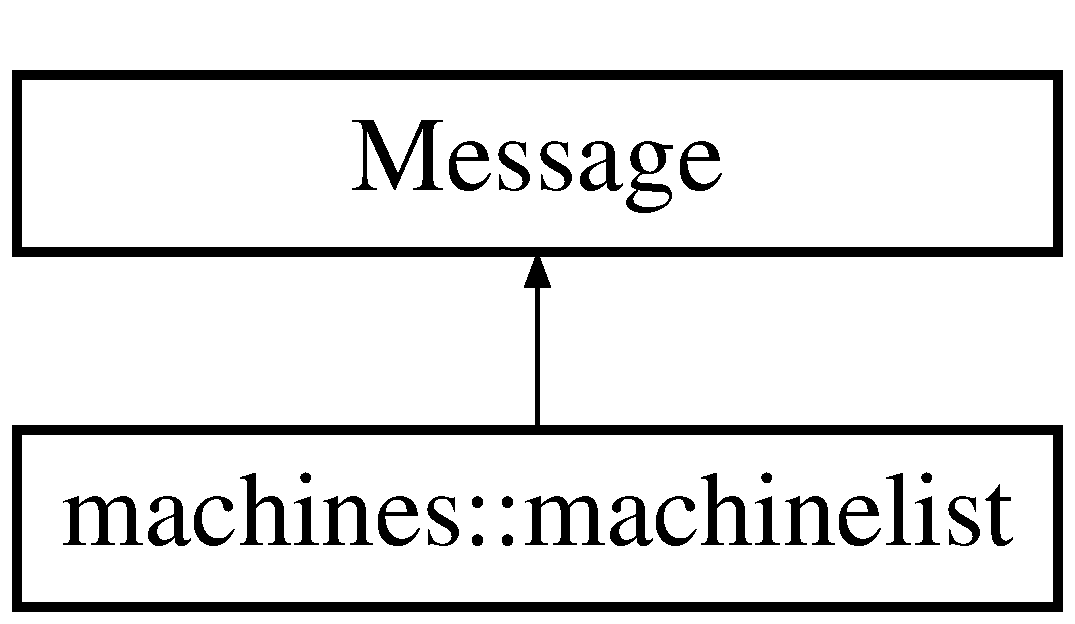
\includegraphics[height=2.000000cm]{classmachines_1_1machinelist}
\end{center}
\end{figure}
\subsection*{Public Member Functions}
\begin{DoxyCompactItemize}
\item 
{\bfseries machinelist} (const \hyperlink{classmachines_1_1machinelist}{machinelist} \&from)\hypertarget{classmachines_1_1machinelist_aeb77751467dab731912ff100d2e8ff8f}{}\label{classmachines_1_1machinelist_aeb77751467dab731912ff100d2e8ff8f}

\item 
\hyperlink{classmachines_1_1machinelist}{machinelist} \& {\bfseries operator=} (const \hyperlink{classmachines_1_1machinelist}{machinelist} \&from)\hypertarget{classmachines_1_1machinelist_a425169f4038ffa9f436a99d131ef65fb}{}\label{classmachines_1_1machinelist_a425169f4038ffa9f436a99d131ef65fb}

\item 
const \+::google\+::protobuf\+::\+Unknown\+Field\+Set \& {\bfseries unknown\+\_\+fields} () const \hypertarget{classmachines_1_1machinelist_a61f5604abcfb838ef755c27de2235a80}{}\label{classmachines_1_1machinelist_a61f5604abcfb838ef755c27de2235a80}

\item 
inline\+::google\+::protobuf\+::\+Unknown\+Field\+Set $\ast$ {\bfseries mutable\+\_\+unknown\+\_\+fields} ()\hypertarget{classmachines_1_1machinelist_a9b509425f813d9287194f5e218a653a3}{}\label{classmachines_1_1machinelist_a9b509425f813d9287194f5e218a653a3}

\item 
void {\bfseries Swap} (\hyperlink{classmachines_1_1machinelist}{machinelist} $\ast$other)\hypertarget{classmachines_1_1machinelist_a18768daa99eec22cc9d0289cc796091f}{}\label{classmachines_1_1machinelist_a18768daa99eec22cc9d0289cc796091f}

\item 
\hyperlink{classmachines_1_1machinelist}{machinelist} $\ast$ {\bfseries New} () const \hypertarget{classmachines_1_1machinelist_a7fed1795d25c11f71312461ada39eaee}{}\label{classmachines_1_1machinelist_a7fed1795d25c11f71312461ada39eaee}

\item 
\hyperlink{classmachines_1_1machinelist}{machinelist} $\ast$ {\bfseries New} (\+::google\+::protobuf\+::\+Arena $\ast$arena) const \hypertarget{classmachines_1_1machinelist_a316522d7c5152bb4564c027dc0fdbe8a}{}\label{classmachines_1_1machinelist_a316522d7c5152bb4564c027dc0fdbe8a}

\item 
void {\bfseries Copy\+From} (const \+::google\+::protobuf\+::\+Message \&from)\hypertarget{classmachines_1_1machinelist_a0c71c10f5fa4b0bc27e2d9391390989c}{}\label{classmachines_1_1machinelist_a0c71c10f5fa4b0bc27e2d9391390989c}

\item 
void {\bfseries Merge\+From} (const \+::google\+::protobuf\+::\+Message \&from)\hypertarget{classmachines_1_1machinelist_a62f63ba0763749be29e474c442278c7e}{}\label{classmachines_1_1machinelist_a62f63ba0763749be29e474c442278c7e}

\item 
void {\bfseries Copy\+From} (const \hyperlink{classmachines_1_1machinelist}{machinelist} \&from)\hypertarget{classmachines_1_1machinelist_a8a33c2bf4c500cb522a8c53a7d64cc52}{}\label{classmachines_1_1machinelist_a8a33c2bf4c500cb522a8c53a7d64cc52}

\item 
void {\bfseries Merge\+From} (const \hyperlink{classmachines_1_1machinelist}{machinelist} \&from)\hypertarget{classmachines_1_1machinelist_a05e4bd84e79d8bbbe89fa1a2862f0f2e}{}\label{classmachines_1_1machinelist_a05e4bd84e79d8bbbe89fa1a2862f0f2e}

\item 
void {\bfseries Clear} ()\hypertarget{classmachines_1_1machinelist_a5f678f33985b00a024ac236c9183cc58}{}\label{classmachines_1_1machinelist_a5f678f33985b00a024ac236c9183cc58}

\item 
bool {\bfseries Is\+Initialized} () const \hypertarget{classmachines_1_1machinelist_a492155d49225019237ef7064c64ff670}{}\label{classmachines_1_1machinelist_a492155d49225019237ef7064c64ff670}

\item 
int {\bfseries Byte\+Size} () const \hypertarget{classmachines_1_1machinelist_ad709a4a55106ea019e42eed22625db49}{}\label{classmachines_1_1machinelist_ad709a4a55106ea019e42eed22625db49}

\item 
bool {\bfseries Merge\+Partial\+From\+Coded\+Stream} (\+::google\+::protobuf\+::io\+::\+Coded\+Input\+Stream $\ast$input)\hypertarget{classmachines_1_1machinelist_a09677a174779b289c58dbf62c479101e}{}\label{classmachines_1_1machinelist_a09677a174779b289c58dbf62c479101e}

\item 
void {\bfseries Serialize\+With\+Cached\+Sizes} (\+::google\+::protobuf\+::io\+::\+Coded\+Output\+Stream $\ast$output) const \hypertarget{classmachines_1_1machinelist_a447136b85daa916e3153b9330ebbcb20}{}\label{classmachines_1_1machinelist_a447136b85daa916e3153b9330ebbcb20}

\item 
\+::google\+::protobuf\+::uint8 $\ast$ {\bfseries Serialize\+With\+Cached\+Sizes\+To\+Array} (\+::google\+::protobuf\+::uint8 $\ast$output) const \hypertarget{classmachines_1_1machinelist_a04bd905536c6df6d42d76e349a97f561}{}\label{classmachines_1_1machinelist_a04bd905536c6df6d42d76e349a97f561}

\item 
int {\bfseries Get\+Cached\+Size} () const \hypertarget{classmachines_1_1machinelist_aff60075cd222fb701216d18d6829d882}{}\label{classmachines_1_1machinelist_aff60075cd222fb701216d18d6829d882}

\item 
\+::google\+::protobuf\+::\+Metadata {\bfseries Get\+Metadata} () const \hypertarget{classmachines_1_1machinelist_a8eed61afd4c0f02caecb24a4196dc2ce}{}\label{classmachines_1_1machinelist_a8eed61afd4c0f02caecb24a4196dc2ce}

\item 
int {\bfseries machine\+\_\+size} () const \hypertarget{classmachines_1_1machinelist_a510f4af329708690aff88485d693969c}{}\label{classmachines_1_1machinelist_a510f4af329708690aff88485d693969c}

\item 
void {\bfseries clear\+\_\+machine} ()\hypertarget{classmachines_1_1machinelist_ad7becd9ea5e7e6fd3ba2d7fa8b2afea3}{}\label{classmachines_1_1machinelist_ad7becd9ea5e7e6fd3ba2d7fa8b2afea3}

\item 
const \+::\hyperlink{classmachines_1_1Machine}{machines\+::\+Machine} \& {\bfseries machine} (int index) const \hypertarget{classmachines_1_1machinelist_a629756ed1e1237f7559bd0bde3204f87}{}\label{classmachines_1_1machinelist_a629756ed1e1237f7559bd0bde3204f87}

\item 
\+::\hyperlink{classmachines_1_1Machine}{machines\+::\+Machine} $\ast$ {\bfseries mutable\+\_\+machine} (int index)\hypertarget{classmachines_1_1machinelist_a63425cd579b78f212451cdc428e745ff}{}\label{classmachines_1_1machinelist_a63425cd579b78f212451cdc428e745ff}

\item 
\+::\hyperlink{classmachines_1_1Machine}{machines\+::\+Machine} $\ast$ {\bfseries add\+\_\+machine} ()\hypertarget{classmachines_1_1machinelist_aa62e554f3e471d13fc1b3f520d504aea}{}\label{classmachines_1_1machinelist_aa62e554f3e471d13fc1b3f520d504aea}

\item 
\+::google\+::protobuf\+::\+Repeated\+Ptr\+Field$<$ \+::\hyperlink{classmachines_1_1Machine}{machines\+::\+Machine} $>$ $\ast$ {\bfseries mutable\+\_\+machine} ()\hypertarget{classmachines_1_1machinelist_a65e0b020a745693c72bc34b820069eb2}{}\label{classmachines_1_1machinelist_a65e0b020a745693c72bc34b820069eb2}

\item 
const \+::google\+::protobuf\+::\+Repeated\+Ptr\+Field$<$ \+::\hyperlink{classmachines_1_1Machine}{machines\+::\+Machine} $>$ \& {\bfseries machine} () const \hypertarget{classmachines_1_1machinelist_a45f99c78c4cb6b6211ad7ad34ebcf6ed}{}\label{classmachines_1_1machinelist_a45f99c78c4cb6b6211ad7ad34ebcf6ed}

\end{DoxyCompactItemize}
\subsection*{Static Public Member Functions}
\begin{DoxyCompactItemize}
\item 
static const \+::google\+::protobuf\+::\+Descriptor $\ast$ {\bfseries descriptor} ()\hypertarget{classmachines_1_1machinelist_a2c61c1349537c46fa0d6ba2e499d6c83}{}\label{classmachines_1_1machinelist_a2c61c1349537c46fa0d6ba2e499d6c83}

\item 
static const \hyperlink{classmachines_1_1machinelist}{machinelist} \& {\bfseries default\+\_\+instance} ()\hypertarget{classmachines_1_1machinelist_a81dd449197eff541e427d328dffdc0a6}{}\label{classmachines_1_1machinelist_a81dd449197eff541e427d328dffdc0a6}

\end{DoxyCompactItemize}
\subsection*{Static Public Attributes}
\begin{DoxyCompactItemize}
\item 
static const int {\bfseries k\+Machine\+Field\+Number} = 1\hypertarget{classmachines_1_1machinelist_a25e357cfdda5b8c035e6ea085a029ae6}{}\label{classmachines_1_1machinelist_a25e357cfdda5b8c035e6ea085a029ae6}

\end{DoxyCompactItemize}
\subsection*{Friends}
\begin{DoxyCompactItemize}
\item 
void {\bfseries protobuf\+\_\+\+Add\+Desc\+\_\+\+Machine\+\_\+2eproto} ()\hypertarget{classmachines_1_1machinelist_ab588f006d8ec48121b79de6050e1f8a3}{}\label{classmachines_1_1machinelist_ab588f006d8ec48121b79de6050e1f8a3}

\item 
void {\bfseries protobuf\+\_\+\+Assign\+Desc\+\_\+\+Machine\+\_\+2eproto} ()\hypertarget{classmachines_1_1machinelist_a4615177ebb310c1aa54ad33e1bf40d43}{}\label{classmachines_1_1machinelist_a4615177ebb310c1aa54ad33e1bf40d43}

\item 
void {\bfseries protobuf\+\_\+\+Shutdown\+File\+\_\+\+Machine\+\_\+2eproto} ()\hypertarget{classmachines_1_1machinelist_abdd3c852817cdd7a28aeb79f6757bde2}{}\label{classmachines_1_1machinelist_abdd3c852817cdd7a28aeb79f6757bde2}

\end{DoxyCompactItemize}


The documentation for this class was generated from the following files\+:\begin{DoxyCompactItemize}
\item 
Machine.\+pb.\+h\item 
Machine.\+pb.\+cc\end{DoxyCompactItemize}

\hypertarget{classMachinetype1}{}\section{Machinetype1 Class Reference}
\label{classMachinetype1}\index{Machinetype1@{Machinetype1}}
Inheritance diagram for Machinetype1\+:\begin{figure}[H]
\begin{center}
\leavevmode
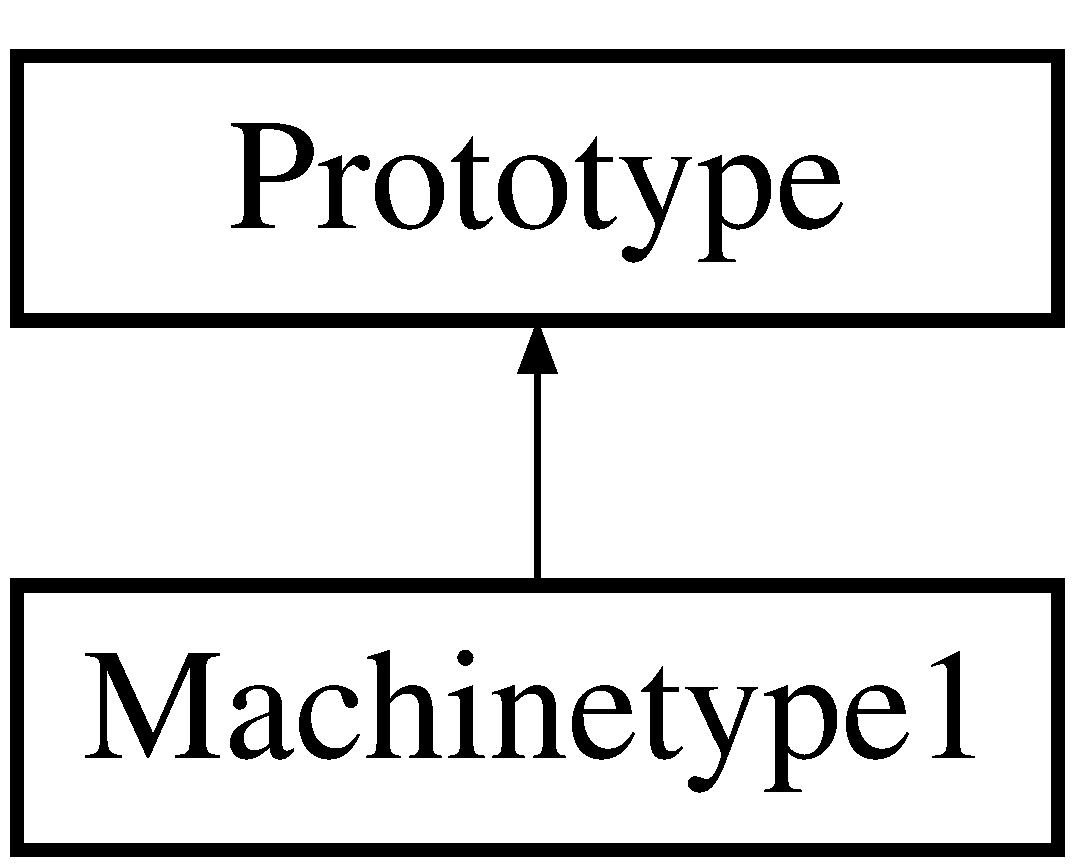
\includegraphics[height=2.000000cm]{classMachinetype1}
\end{center}
\end{figure}
\subsection*{Public Member Functions}
\begin{DoxyCompactItemize}
\item 
{\bfseries Machinetype1} (string utype, string ID)\hypertarget{classMachinetype1_a6115ce5e071ca63100700b98cfe74a92}{}\label{classMachinetype1_a6115ce5e071ca63100700b98cfe74a92}

\item 
\hyperlink{classPrototype}{Prototype} $\ast$ \hyperlink{classMachinetype1_a5f2b94ac7f57e3120a5abf21519b3e74}{clone} ()
\item 
string {\bfseries get\+Type} ()\hypertarget{classMachinetype1_a9482930efc9d0bc0bf5c952b723ec526}{}\label{classMachinetype1_a9482930efc9d0bc0bf5c952b723ec526}

\item 
string {\bfseries get\+Name} ()\hypertarget{classMachinetype1_aa2f384411cfaa25d2348fbd6a19f4bee}{}\label{classMachinetype1_aa2f384411cfaa25d2348fbd6a19f4bee}

\item 
void {\bfseries set\+Name} (string Name)\hypertarget{classMachinetype1_a51d81bf04ef5aea0b3083b1389a2659e}{}\label{classMachinetype1_a51d81bf04ef5aea0b3083b1389a2659e}

\item 
void {\bfseries set\+Type} (string \hyperlink{classPrototype_a2d6c59c7f19020c5c66bb1902d858992}{type})\hypertarget{classMachinetype1_ae6639a21253034a2d73cfccc20b04f47}{}\label{classMachinetype1_ae6639a21253034a2d73cfccc20b04f47}

\end{DoxyCompactItemize}
\subsection*{Additional Inherited Members}


\subsection{Member Function Documentation}
\index{Machinetype1@{Machinetype1}!clone@{clone}}
\index{clone@{clone}!Machinetype1@{Machinetype1}}
\subsubsection[{clone()}]{\setlength{\rightskip}{0pt plus 5cm}{\bf Prototype}$\ast$ Machinetype1\+::clone (
\begin{DoxyParamCaption}
{}
\end{DoxyParamCaption}
)\hspace{0.3cm}{\ttfamily [inline]}, {\ttfamily [virtual]}}\hypertarget{classMachinetype1_a5f2b94ac7f57e3120a5abf21519b3e74}{}\label{classMachinetype1_a5f2b94ac7f57e3120a5abf21519b3e74}
Function declarations for prototype 

Implements \hyperlink{classPrototype_ab1ea90138cda9e68f368ebe8711428e7}{Prototype}.



The documentation for this class was generated from the following file\+:\begin{DoxyCompactItemize}
\item 
main.\+cpp\end{DoxyCompactItemize}

\hypertarget{classMachinetype2}{}\section{Machinetype2 Class Reference}
\label{classMachinetype2}\index{Machinetype2@{Machinetype2}}
Inheritance diagram for Machinetype2\+:\begin{figure}[H]
\begin{center}
\leavevmode
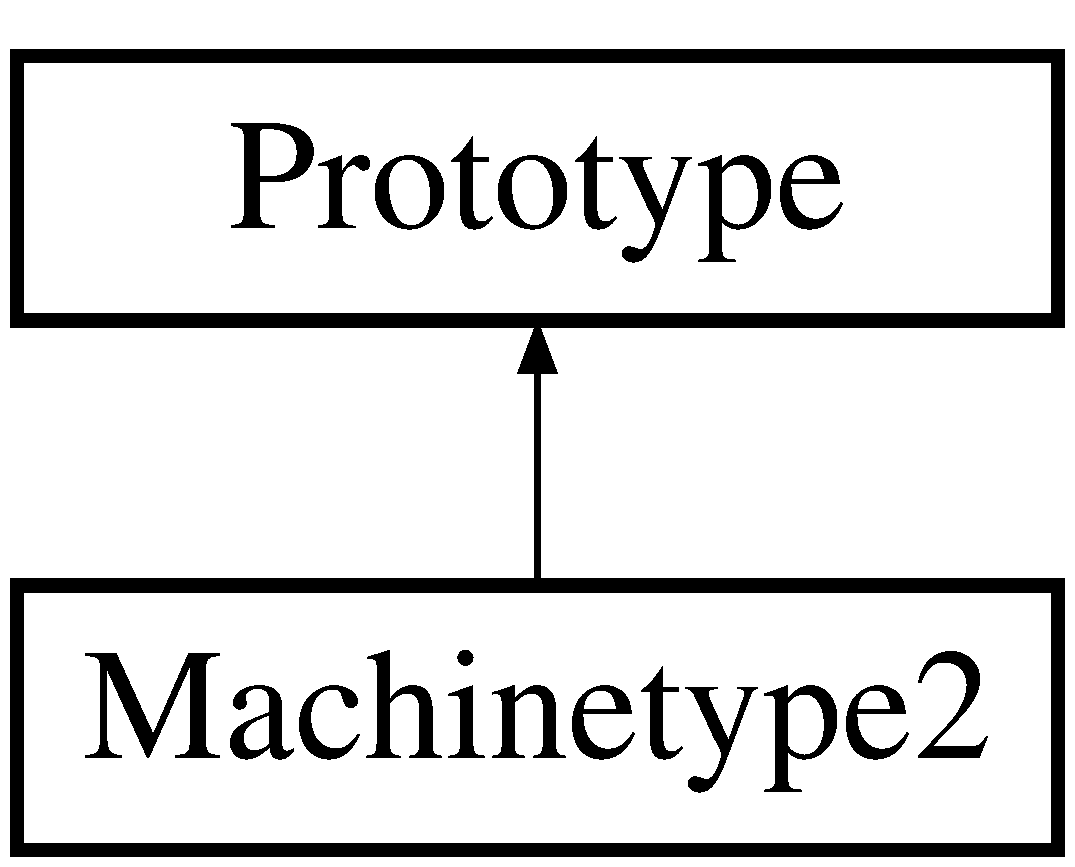
\includegraphics[height=2.000000cm]{classMachinetype2}
\end{center}
\end{figure}
\subsection*{Public Member Functions}
\begin{DoxyCompactItemize}
\item 
{\bfseries Machinetype2} (string utype, string ID)\hypertarget{classMachinetype2_ae858e194de2a36f88ae70cde70208829}{}\label{classMachinetype2_ae858e194de2a36f88ae70cde70208829}

\item 
\hyperlink{classPrototype}{Prototype} $\ast$ \hyperlink{classMachinetype2_a90dbc90692c2890c1afb2b5ff130987b}{clone} ()
\item 
string {\bfseries get\+Type} ()\hypertarget{classMachinetype2_a866af4748f21efcc111ab6d674e689f4}{}\label{classMachinetype2_a866af4748f21efcc111ab6d674e689f4}

\item 
string {\bfseries get\+Name} ()\hypertarget{classMachinetype2_ab1330110821d06d6947f976c3fa47c8c}{}\label{classMachinetype2_ab1330110821d06d6947f976c3fa47c8c}

\item 
void {\bfseries set\+Name} (string Name)\hypertarget{classMachinetype2_aca1fc24b86786ba7f55e6d8b590bd4f2}{}\label{classMachinetype2_aca1fc24b86786ba7f55e6d8b590bd4f2}

\item 
void {\bfseries set\+Type} (string \hyperlink{classPrototype_a2d6c59c7f19020c5c66bb1902d858992}{type})\hypertarget{classMachinetype2_a8992165a2de7596fefc6b9b1e96f79ce}{}\label{classMachinetype2_a8992165a2de7596fefc6b9b1e96f79ce}

\end{DoxyCompactItemize}
\subsection*{Additional Inherited Members}


\subsection{Detailed Description}
Type 2 of machine cloned via prototype 

\subsection{Member Function Documentation}
\index{Machinetype2@{Machinetype2}!clone@{clone}}
\index{clone@{clone}!Machinetype2@{Machinetype2}}
\subsubsection[{clone()}]{\setlength{\rightskip}{0pt plus 5cm}{\bf Prototype}$\ast$ Machinetype2\+::clone (
\begin{DoxyParamCaption}
{}
\end{DoxyParamCaption}
)\hspace{0.3cm}{\ttfamily [inline]}, {\ttfamily [virtual]}}\hypertarget{classMachinetype2_a90dbc90692c2890c1afb2b5ff130987b}{}\label{classMachinetype2_a90dbc90692c2890c1afb2b5ff130987b}
Function declarations for prototype 

Implements \hyperlink{classPrototype_ab1ea90138cda9e68f368ebe8711428e7}{Prototype}.



The documentation for this class was generated from the following file\+:\begin{DoxyCompactItemize}
\item 
main.\+cpp\end{DoxyCompactItemize}

\hypertarget{classPrototype}{}\section{Prototype Class Reference}
\label{classPrototype}\index{Prototype@{Prototype}}


\hyperlink{classPrototype}{Prototype} class.  


Inheritance diagram for Prototype\+:\begin{figure}[H]
\begin{center}
\leavevmode
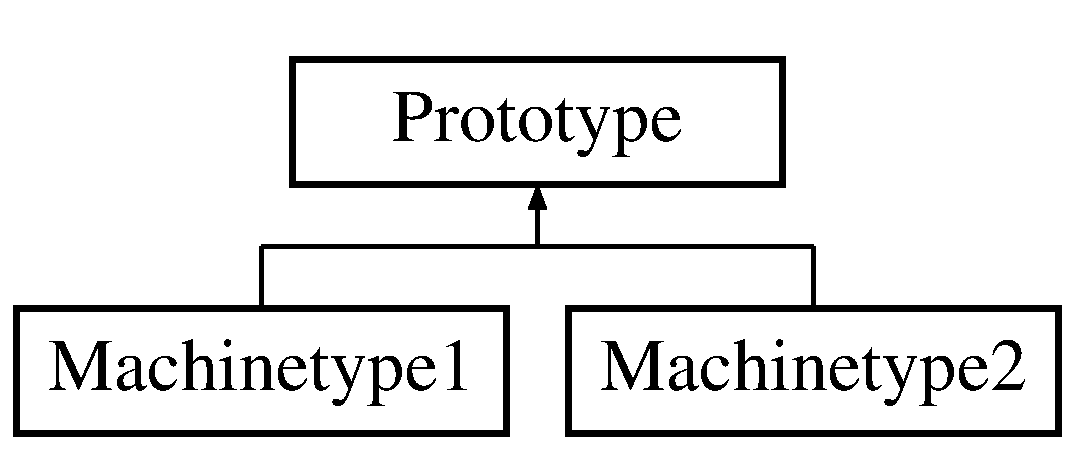
\includegraphics[height=2.000000cm]{classPrototype}
\end{center}
\end{figure}
\subsection*{Public Member Functions}
\begin{DoxyCompactItemize}
\item 
virtual \hyperlink{classPrototype}{Prototype} $\ast$ \hyperlink{classPrototype_ab1ea90138cda9e68f368ebe8711428e7}{clone} ()=0
\item 
string \hyperlink{classPrototype_aaeb405998fccb4777c2651dfe2361628}{get\+Type} ()
\item 
string \hyperlink{classPrototype_a3a24a2b64dc329301c971e35adac4cc4}{get\+Name} ()
\item 
void \hyperlink{classPrototype_a5198d9e7e0dcd775c15111a719060f02}{set\+Type} (string \hyperlink{classPrototype_a2d6c59c7f19020c5c66bb1902d858992}{type})
\item 
void \hyperlink{classPrototype_a041609c27bad74826c98e6e4b0c78601}{set\+Name} (string Name)
\end{DoxyCompactItemize}
\subsection*{Protected Attributes}
\begin{DoxyCompactItemize}
\item 
string \hyperlink{classPrototype_a2d6c59c7f19020c5c66bb1902d858992}{type}
\item 
string {\bfseries name}\hypertarget{classPrototype_aa3f0d066a86e518800f81f760884a681}{}\label{classPrototype_aa3f0d066a86e518800f81f760884a681}

\end{DoxyCompactItemize}


\subsection{Detailed Description}
\hyperlink{classPrototype}{Prototype} class. 

Basis for making new machines. 

\subsection{Member Function Documentation}
\index{Prototype@{Prototype}!clone@{clone}}
\index{clone@{clone}!Prototype@{Prototype}}
\subsubsection[{clone()=0}]{\setlength{\rightskip}{0pt plus 5cm}virtual {\bf Prototype}$\ast$ Prototype\+::clone (
\begin{DoxyParamCaption}
{}
\end{DoxyParamCaption}
)\hspace{0.3cm}{\ttfamily [pure virtual]}}\hypertarget{classPrototype_ab1ea90138cda9e68f368ebe8711428e7}{}\label{classPrototype_ab1ea90138cda9e68f368ebe8711428e7}
Function declarations for prototype 

Implemented in \hyperlink{classMachinetype2_a90dbc90692c2890c1afb2b5ff130987b}{Machinetype2}, and \hyperlink{classMachinetype1_a5f2b94ac7f57e3120a5abf21519b3e74}{Machinetype1}.

\index{Prototype@{Prototype}!get\+Name@{get\+Name}}
\index{get\+Name@{get\+Name}!Prototype@{Prototype}}
\subsubsection[{get\+Name()}]{\setlength{\rightskip}{0pt plus 5cm}string Prototype\+::get\+Name (
\begin{DoxyParamCaption}
{}
\end{DoxyParamCaption}
)\hspace{0.3cm}{\ttfamily [inline]}}\hypertarget{classPrototype_a3a24a2b64dc329301c971e35adac4cc4}{}\label{classPrototype_a3a24a2b64dc329301c971e35adac4cc4}
Getter for name(\+I\+D) value \index{Prototype@{Prototype}!get\+Type@{get\+Type}}
\index{get\+Type@{get\+Type}!Prototype@{Prototype}}
\subsubsection[{get\+Type()}]{\setlength{\rightskip}{0pt plus 5cm}string Prototype\+::get\+Type (
\begin{DoxyParamCaption}
{}
\end{DoxyParamCaption}
)\hspace{0.3cm}{\ttfamily [inline]}}\hypertarget{classPrototype_aaeb405998fccb4777c2651dfe2361628}{}\label{classPrototype_aaeb405998fccb4777c2651dfe2361628}
Getters for the type \index{Prototype@{Prototype}!set\+Name@{set\+Name}}
\index{set\+Name@{set\+Name}!Prototype@{Prototype}}
\subsubsection[{set\+Name(string Name)}]{\setlength{\rightskip}{0pt plus 5cm}void Prototype\+::set\+Name (
\begin{DoxyParamCaption}
\item[{string}]{Name}
\end{DoxyParamCaption}
)\hspace{0.3cm}{\ttfamily [inline]}}\hypertarget{classPrototype_a041609c27bad74826c98e6e4b0c78601}{}\label{classPrototype_a041609c27bad74826c98e6e4b0c78601}
Setter for name for prototype \index{Prototype@{Prototype}!set\+Type@{set\+Type}}
\index{set\+Type@{set\+Type}!Prototype@{Prototype}}
\subsubsection[{set\+Type(string type)}]{\setlength{\rightskip}{0pt plus 5cm}void Prototype\+::set\+Type (
\begin{DoxyParamCaption}
\item[{string}]{type}
\end{DoxyParamCaption}
)\hspace{0.3cm}{\ttfamily [inline]}}\hypertarget{classPrototype_a5198d9e7e0dcd775c15111a719060f02}{}\label{classPrototype_a5198d9e7e0dcd775c15111a719060f02}
Setters for the name and the type 

\subsection{Member Data Documentation}
\index{Prototype@{Prototype}!type@{type}}
\index{type@{type}!Prototype@{Prototype}}
\subsubsection[{type}]{\setlength{\rightskip}{0pt plus 5cm}string Prototype\+::type\hspace{0.3cm}{\ttfamily [protected]}}\hypertarget{classPrototype_a2d6c59c7f19020c5c66bb1902d858992}{}\label{classPrototype_a2d6c59c7f19020c5c66bb1902d858992}
Variable delcarations for prototype 

The documentation for this class was generated from the following file\+:\begin{DoxyCompactItemize}
\item 
main.\+cpp\end{DoxyCompactItemize}

\hypertarget{structmachines_1_1StaticDescriptorInitializer__Machine__2eproto}{}\section{machines\+:\+:Static\+Descriptor\+Initializer\+\_\+\+Machine\+\_\+2eproto Struct Reference}
\label{structmachines_1_1StaticDescriptorInitializer__Machine__2eproto}\index{machines\+::\+Static\+Descriptor\+Initializer\+\_\+\+Machine\+\_\+2eproto@{machines\+::\+Static\+Descriptor\+Initializer\+\_\+\+Machine\+\_\+2eproto}}


The documentation for this struct was generated from the following file\+:\begin{DoxyCompactItemize}
\item 
Machine.\+pb.\+cc\end{DoxyCompactItemize}

%--- End generated contents ---

% Index
\backmatter
\newpage
\phantomsection
\clearemptydoublepage
\addcontentsline{toc}{chapter}{Index}
\printindex

\end{document}
